\documentclass[border=4pt]{standalone}
\usepackage{tikz}
\usetikzlibrary{positioning, arrows.meta}
\usepackage{xcolor}

\definecolor{regHigh}{HTML}{27AE60}
\definecolor{regMed}{HTML}{E67E22}
\definecolor{regLow}{HTML}{E74C3C}
\definecolor{grayDark}{HTML}{4A5568}
\definecolor{barBg}{HTML}{F1F4F8}

\begin{document}
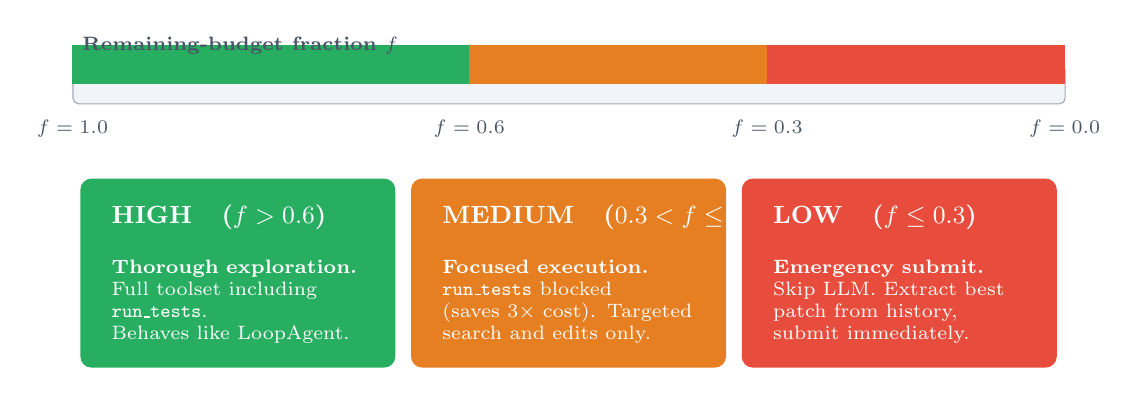
\begin{tikzpicture}[
    reg/.style={rectangle, rounded corners=4pt, minimum height=2.4cm, minimum width=4cm,
                draw=none, align=left, font=\small, inner sep=8pt},
    title/.style={font=\bfseries\small, text=white},
    body/.style={font=\scriptsize, text=grayDark, align=left}
  ]

  % Budget bar at top
  \node[draw=grayDark!50, rounded corners=2pt, fill=barBg, minimum width=12.6cm,
        minimum height=0.5cm, anchor=west] (bar) at (0,3.0) {};
  \fill[regHigh] ([xshift=0pt]bar.west) rectangle ([xshift=5.04cm,yshift=0.5cm]bar.west);
  \fill[regMed]  ([xshift=5.04cm]bar.west) rectangle ([xshift=8.82cm,yshift=0.5cm]bar.west);
  \fill[regLow]  ([xshift=8.82cm]bar.west) rectangle ([xshift=12.6cm,yshift=0.5cm]bar.west);

  \node[font=\scriptsize, text=grayDark, anchor=north] at ([yshift=-2pt]bar.south west) {$f=1.0$};
  \node[font=\scriptsize, text=grayDark, anchor=north] at ([xshift=5.04cm,yshift=-2pt]bar.south west) {$f=0.6$};
  \node[font=\scriptsize, text=grayDark, anchor=north] at ([xshift=8.82cm,yshift=-2pt]bar.south west) {$f=0.3$};
  \node[font=\scriptsize, text=grayDark, anchor=north] at ([xshift=12.6cm,yshift=-2pt]bar.south west) {$f=0.0$};
  \node[font=\scriptsize\bfseries, text=grayDark, anchor=south west] at (bar.north west) {Remaining-budget fraction $f$};

  % Three regime cards
  \node[reg, fill=regHigh] (H) at (2.1,0.6) {};
  \node[title, anchor=north west] at ([xshift=8pt,yshift=-6pt]H.north west) {HIGH ~ ($f > 0.6$)};
  \node[body, anchor=north west, text width=3.4cm] at ([xshift=8pt,yshift=-26pt]H.north west)
       {\textcolor{white}{\textbf{Thorough exploration.}\\
        Full toolset including \texttt{run\_tests}.\\
        Behaves like LoopAgent.}};

  \node[reg, fill=regMed] (M) at (6.3,0.6) {};
  \node[title, anchor=north west] at ([xshift=8pt,yshift=-6pt]M.north west) {MEDIUM ~ ($0.3 < f \leq 0.6$)};
  \node[body, anchor=north west, text width=3.4cm] at ([xshift=8pt,yshift=-26pt]M.north west)
       {\textcolor{white}{\textbf{Focused execution.}\\
        \texttt{run\_tests} blocked\\
        (saves $3\times$ cost). Targeted\\
        search and edits only.}};

  \node[reg, fill=regLow] (L) at (10.5,0.6) {};
  \node[title, anchor=north west] at ([xshift=8pt,yshift=-6pt]L.north west) {LOW ~ ($f \leq 0.3$)};
  \node[body, anchor=north west, text width=3.4cm] at ([xshift=8pt,yshift=-26pt]L.north west)
       {\textcolor{white}{\textbf{Emergency submit.}\\
        Skip LLM. Extract best\\
        patch from history,\\
        submit immediately.}};

\end{tikzpicture}
\end{document}
